\begin{frame}
  \frametitle{Metadaten - Vorratsdatenspeicherung}
  \begin{itemize}
    \item Handynetz
      \begin{itemize}
        \item Telefonnummern
        \item Zeitpunkt und Dauer (Telefonate, SMS)
        \item Funkzelle (Ort)
      \end{itemize}
    \item Internet
      \begin{itemize}
        \item IP-Adresse (= ungefährer Ort)
        \item Alle Verbindungen
        \item Email: Adressen von Sender und Empfänger, Zugriff
      \end{itemize}
  \end{itemize}
\end{frame}

\note{Metadaten sind alles außer Inhaltsdaten. Man kann nach ihnen mit den W-Fragen fragen: WER hat etwas WANN und WIE gemacht und WO hat er sich dabei befunden. Die Vorratsdatenspeicherung, die in Deutschland und der EU sehr umstritten ist (aktuellen Stand darlegen) sammelt genau solche Daten (siehe Folie). Wir wollen im Folgenden zeigen, dass man mit Metadaten viel mehr über eine Person herausfinden kann als mit Gesprächsinhalten und damit auch zeigen, wieso wir die VDS für eine schlechte Idee halten.}

\begin{frame}
    \frametitle{Metadaten - VDS}
    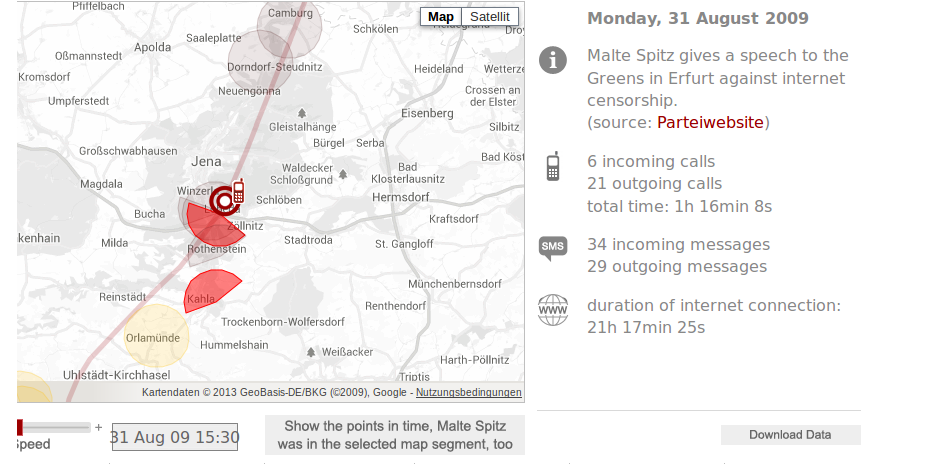
\includegraphics[height=0.7\textheight]{img/maltespitz.png}
\end{frame}

\note{Malte Spitz ist im Vorstand der Grünen. Er hat sich, als es die Vorratsdatenspeicherung eine Weile gab, seine Daten von der Telekom erklagt und Zeit Online hat sie visualisiert. Man kann ihm über Monate weg ``folgen'', sieht wo er war, ggf. mit wem er sich getroffen hat, zu welchen Ärzten er gegangen ist und wann er auf Arbeit war.}
